% ============================================================================
% Lecture 02 (B01): Why Deep Learning for Economics and Finance?
% Deep Learning for Solving and Estimating Dynamic Models in Economics and Finance
% Course author: Simon Scheidegger
% ============================================================================

\documentclass[aspectratio=169,11pt]{beamer}

% ---------- Theme and colors ----------
\usecolortheme{dove}
\setbeamertemplate{navigation symbols}{}
\setbeamertemplate{footline}{%
  \hfill\usebeamerfont{page number in head/foot}%
  \usebeamercolor[fg]{normal text}%
  \insertframenumber\,/\,\inserttotalframenumber\kern1em\vskip4pt}
\setbeamerfont{frametitle}{size=\huge}

% ---------- Packages ----------
\usepackage[utf8]{inputenc}
\usepackage[T1]{fontenc}
\usepackage{amsmath,amssymb,amsfonts}
\usepackage{bm}
\usepackage{graphicx}
\usepackage{tikz}
\usetikzlibrary{shapes,arrows.meta,positioning,calc,fit,backgrounds,patterns,decorations.pathreplacing}
\usepackage{pgfplots}
\pgfplotsset{compat=1.18}
\usepackage{booktabs}
\usepackage{hyperref}
\usepackage{multicol}
\usepackage{xcolor}
\usepackage{algorithm}
\usepackage{algorithmic}

% ---------- Custom colors ----------
\definecolor{uzhblue}{rgb}{0,0,0.5}
\definecolor{uzhgreylight}{RGB}{236,238,241}
\definecolor{uzhgreydark}{RGB}{81,86,94}
\definecolor{harvardcrimson}{RGB}{153,0,0}
\definecolor{unil@blue}{RGB}{0,140,204}
\definecolor{unil@black}{RGB}{35,31,32}
\definecolor{darkgreen}{RGB}{0,100,0}
\definecolor{darkred}{RGB}{139,0,0}
\definecolor{softblue}{RGB}{70,130,180}
\definecolor{softorange}{RGB}{230,159,0}
\definecolor{softgreen}{RGB}{0,158,115}

% ---------- Set beamer colors ----------
\setbeamercolor{frametitle}{bg=uzhgreylight, fg=uzhblue}
\setbeamercolor{title}{fg=uzhblue}
\setbeamercolor{structure}{fg=uzhblue}
\setbeamercolor{block title}{bg=unil@blue, fg=white}
\setbeamercolor{block body}{bg=uzhgreylight}
\setbeamercolor{block title alerted}{bg=darkred,fg=white}
\setbeamercolor{block body alerted}{bg=red!5}
\setbeamercolor{block title example}{bg=darkgreen,fg=white}
\setbeamercolor{block body example}{bg=green!5}
\setbeamercolor{item}{fg=unil@black}
\setbeamercolor{normal text}{fg=unil@black}

% ---------- Emphasis and hyperlinks ----------
\newcommand{\emphc}[1]{\textcolor{harvardcrimson}{#1}}
\hypersetup{colorlinks,linkcolor=harvardcrimson,urlcolor=harvardcrimson}

% ---------- Math commands ----------
\newcommand{\x}{\bm{x}}
\newcommand{\w}{\bm{w}}
\newcommand{\bb}{\bm{b}}
\newcommand{\z}{\bm{z}}
\newcommand{\W}{\bm{W}}
\newcommand{\X}{\bm{X}}
\renewcommand{\a}{\bm{a}}
\newcommand{\R}{\mathbb{R}}
\newcommand{\E}[1]{\mathbb{E}\!\left[#1\right]}
\DeclareMathOperator*{\argmin}{arg\,min}
\DeclareMathOperator*{\argmax}{arg\,max}

\title[Lecture 04 (B03)]{Lecture 04 (B03): Generalization and Sequence Models}
\subtitle{Bias-variance, double descent, RNN / LSTM / Transformer}
\author{Simon Scheidegger}
\institute{HEC, University of Lausanne}
\date{}
\begin{document}

{\setbeamercolor{background canvas}{bg=uzhgreylight}
\begin{frame}
\titlepage
\end{frame}
}

% --- About-this-lecture orientation ---
\begin{frame}{About this lecture}
\small
\begin{block}{What this lecture covers}
\begin{itemize}\itemsep2pt
  \item Overfitting vs underfitting, train / validation / test splits
  \item Regularization: $L_2$ penalty, dropout, early stopping; the deep-double-descent surprise
  \item Sequence models: RNNs, LSTMs, attention, the transformer block
\end{itemize}
\end{block}
\begin{block}{Builds on}
\begin{itemize}\itemsep2pt
  \item Lecture 03 (training neural networks)
\end{itemize}
\end{block}
\begin{block}{Leads to}
\begin{itemize}\itemsep2pt
  \item Lecture 05 (loss design)
  \item Lecture 06+ (DEQNs as a specific architecture)
\end{itemize}
\end{block}
\end{frame}

\begin{frame}{}
\begin{center}
{\Huge \textcolor{uzhblue}{Part IV}}\\[0.8em]
{\LARGE Generalization and Regularization}
\end{center}
\end{frame}

% --- Slide 42: Overfitting ---
\begin{frame}{Overfitting and Underfitting}
\begin{center}
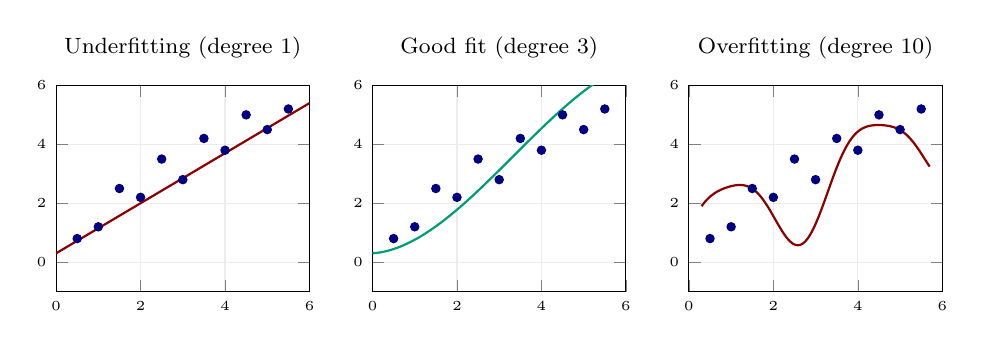
\begin{tikzpicture}
% Panel 1: Underfitting
\begin{axis}[
    name=p1,
    width=4.8cm, height=4.2cm,
    title={\footnotesize Underfitting (degree 1)},
    title style={font=\footnotesize},
    tick label style={font=\tiny},
    xmin=0, xmax=6, ymin=-1, ymax=6,
    grid=major, grid style={gray!15},
]
    \addplot[only marks, mark=*, mark size=1.5pt, uzhblue] coordinates {
        (0.5,0.8) (1,1.2) (1.5,2.5) (2,2.2) (2.5,3.5) (3,2.8) (3.5,4.2) (4,3.8) (4.5,5) (5,4.5) (5.5,5.2)
    };
    \addplot[thick, darkred, domain=0:6, samples=2]{0.3+0.85*x};
\end{axis}

% Panel 2: Good fit
\begin{axis}[
    at={($(p1.east)+(0.8cm,0)$)}, anchor=west,
    name=p2,
    width=4.8cm, height=4.2cm,
    title={\footnotesize Good fit (degree 3)},
    title style={font=\footnotesize},
    tick label style={font=\tiny},
    xmin=0, xmax=6, ymin=-1, ymax=6,
    grid=major, grid style={gray!15},
]
    \addplot[only marks, mark=*, mark size=1.5pt, uzhblue] coordinates {
        (0.5,0.8) (1,1.2) (1.5,2.5) (2,2.2) (2.5,3.5) (3,2.8) (3.5,4.2) (4,3.8) (4.5,5) (5,4.5) (5.5,5.2)
    };
    \addplot[thick, softgreen, domain=0:6, samples=100]{0.3+0.1*x+0.4*x^2-0.04*x^3};
\end{axis}

% Panel 3: Overfitting
\begin{axis}[
    at={($(p2.east)+(0.8cm,0)$)}, anchor=west,
    width=4.8cm, height=4.2cm,
    title={\footnotesize Overfitting (degree 10)},
    title style={font=\footnotesize},
    tick label style={font=\tiny},
    xmin=0, xmax=6, ymin=-1, ymax=6,
    grid=major, grid style={gray!15},
]
    \addplot[only marks, mark=*, mark size=1.5pt, uzhblue] coordinates {
        (0.5,0.8) (1,1.2) (1.5,2.5) (2,2.2) (2.5,3.5) (3,2.8) (3.5,4.2) (4,3.8) (4.5,5) (5,4.5) (5.5,5.2)
    };
    \addplot[thick, darkred, domain=0.3:5.7, samples=200]{
        0.8 + 1.5*sin(deg(x*1.8)) + 0.3*cos(deg(x*3.5)) + 0.6*x
    };
\end{axis}
\end{tikzpicture}
\end{center}

\vspace{0.2cm}
\begin{itemize}
    \item \textbf{Underfitting:} model too simple, high bias, cannot capture the pattern.
    \item \textbf{Overfitting:} model too complex, fits noise, poor generalization to new data.
    \item \textbf{Goal:} find the right complexity that generalizes well.
\end{itemize}
\end{frame}

% --- Slide 43: Train/Val/Test ---
\begin{frame}{Train / Validation / Test Split}
\begin{center}
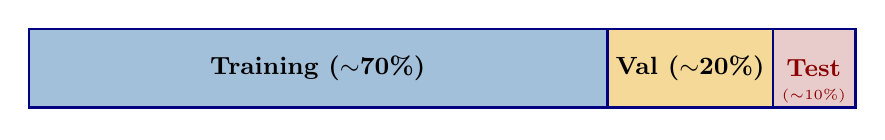
\begin{tikzpicture}
    % Full bar
    \fill[softblue!30] (0,0) rectangle (10.5,1);
    % Train
    \fill[softblue!50] (0,0) rectangle (7.35,1);
    % Val
    \fill[softorange!40] (7.35,0) rectangle (9.45,1);
    % Test
    \fill[darkred!20] (9.45,0) rectangle (10.5,1);
    % Borders
    \draw[uzhblue, thick] (0,0) rectangle (10.5,1);
    \draw[uzhblue, thick] (7.35,0) -- (7.35,1);
    \draw[uzhblue, thick] (9.45,0) -- (9.45,1);
    % Labels
    \node[font=\small\bfseries] at (3.67,0.5) {Training ($\sim$70\%)};
    \node[font=\small\bfseries] at (8.4,0.5) {Val ($\sim$20\%)};
    \node[font=\small\bfseries, darkred] at (9.97,0.5) {Test};
    \node[font=\tiny, darkred] at (9.97,0.15) {($\sim$10\%)};
\end{tikzpicture}
\end{center}

\vspace{0.4cm}
\begin{columns}[T]
\column{0.32\textwidth}
\begin{block}{\centering Training set}
    \centering
    {\small Used to fit model parameters $\bm{\theta}$ via optimization.}
\end{block}

\column{0.32\textwidth}
\begin{block}{\centering Validation set}
    \centering
    {\small Used for model selection: hyperparameters, architecture, early stopping.}
\end{block}

\column{0.32\textwidth}
\begin{block}{\centering Test set}
    \centering
    {\small Touched \textbf{once} at the very end to report final performance.}
\end{block}
\end{columns}

\vspace{0.3cm}
\begin{alertblock}{}
\centering Never use the test set for any decision during model development!
\end{alertblock}
\end{frame}

% --- Regularization Overview (concept map) ---
\begin{frame}{Regularization Techniques --- Overview}
\small
Goal: bias the learner toward \emphc{simpler} hypotheses so it generalizes beyond the training sample.

\vspace{0.3cm}
\begin{center}
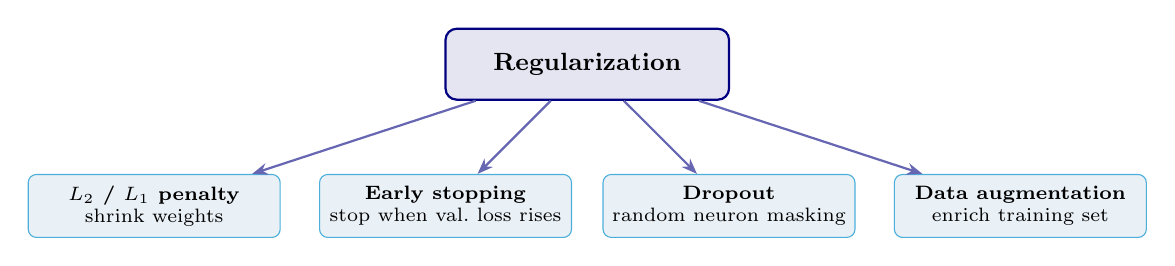
\begin{tikzpicture}[
    root/.style={rectangle, draw=uzhblue, thick, rounded corners=4pt,
                 fill=uzhblue!10, font=\small\bfseries,
                 minimum width=3.6cm, minimum height=0.9cm, align=center},
    leaf/.style={rectangle, draw=unil@blue!70, fill=softblue!12, rounded corners=3pt,
                 font=\scriptsize, minimum width=3.2cm, minimum height=0.8cm,
                 align=center, inner sep=3pt},
    arr/.style={-{Stealth[length=2mm]}, thick, uzhblue!60}
]
    \node[root] (r) at (0,0) {Regularization};
    \node[leaf] (l1) at (-5.5,-1.8) {\textbf{$L_2$ / $L_1$ penalty}\\ shrink weights};
    \node[leaf] (l2) at (-1.8,-1.8) {\textbf{Early stopping}\\ stop when val.\ loss rises};
    \node[leaf] (l3) at (1.8,-1.8) {\textbf{Dropout}\\ random neuron masking};
    \node[leaf] (l4) at (5.5,-1.8) {\textbf{Data augmentation}\\ enrich training set};
    \foreach \n in {l1,l2,l3,l4} \draw[arr] (r) -- (\n);
\end{tikzpicture}
\end{center}

\vspace{0.3cm}
The next slides cover \textbf{early stopping}, \textbf{$L_2$}, and \textbf{dropout} in detail; data augmentation is task-specific (images, time series) and is left as a reading pointer.
\end{frame}

% --- Slide 44: Early Stopping ---
\begin{frame}{Early Stopping}
\begin{columns}[T]
\column{0.48\textwidth}
\begin{center}
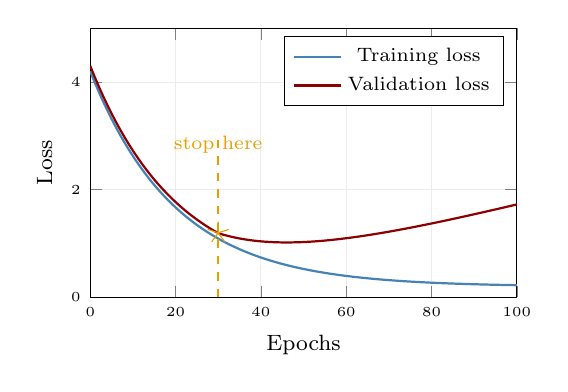
\begin{tikzpicture}
\begin{axis}[
    width=7cm, height=5cm,
    xlabel={Epochs}, ylabel={Loss},
    xlabel style={font=\footnotesize},
    ylabel style={font=\footnotesize},
    tick label style={font=\tiny},
    xmin=0, xmax=100, ymin=0, ymax=5,
    grid=major, grid style={gray!15},
    legend pos=north east,
    legend style={font=\scriptsize},
]
    % Training loss
    \addplot[thick, softblue, domain=0:100, samples=100]{4*exp(-0.05*x)+0.2};
    \addlegendentry{Training loss}
    % Validation loss
    \addplot[thick, darkred, domain=0:100, samples=100]{
        4*exp(-0.05*x) + 0.3 + 0.02*(x-30)*(x>30)
    };
    \addlegendentry{Validation loss}
    % Optimal point
    \draw[softorange, thick, dashed] (axis cs:30,0) -- (axis cs:30,3);
    \node[font=\scriptsize, softorange, above] at (axis cs:30,2.5) {stop here};
    \addplot[only marks, mark=star, mark size=4pt, softorange] coordinates {(30,1.2)};
\end{axis}
\end{tikzpicture}
\end{center}

\column{0.48\textwidth}
\vspace{0.3cm}
\textbf{Idea:} monitor the validation loss during training.  Stop when it starts increasing.

\vspace{0.3cm}
\textbf{In practice:}
\begin{enumerate}
    \item After each epoch, evaluate loss on validation set.
    \item Save model weights whenever validation loss improves.
    \item If no improvement for $p$ consecutive epochs (``patience''), stop training.
    \item Return the saved best weights.
\end{enumerate}

\vspace{0.3cm}
{\small Early stopping is a simple and effective form of regularization.}
\end{columns}
\end{frame}

% --- Slide 45: Regularization ---
\begin{frame}{Regularization: $L_2$ Penalty and Dropout}
\begin{columns}[T]
\column{0.48\textwidth}
\textbf{$L_2$ Regularization (Weight Decay):}

Add a penalty to the loss:
\[
    \tilde{J}(\bm{\theta}) = J(\bm{\theta}) + \frac{\lambda}{2}\|\bm{\theta}\|_2^2
\]
Encourages small weights $\Rightarrow$ simpler model.

\vspace{0.2cm}
\textbf{Dropout} (Srivastava et al., 2014):

During training, randomly zero out each neuron with probability $p$ (typically 0.5). Forces the network not to rely on any single neuron. The standard \emph{inverted dropout} variant divides activations by $(1{-}p)$ during training, so no test-time rescaling is needed.

\column{0.48\textwidth}
\begin{center}
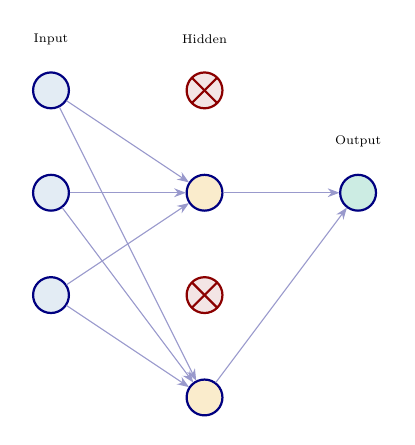
\begin{tikzpicture}[scale=0.65, transform shape,
    neuron/.style={circle, draw=uzhblue, thick, minimum size=7mm},
    dead/.style={circle, draw=darkred, thick, minimum size=7mm, fill=darkred!10,
                 path picture={\draw[darkred,thick] (path picture bounding box.south west)
                 -- (path picture bounding box.north east);
                 \draw[darkred,thick] (path picture bounding box.north west)
                 -- (path picture bounding box.south east);}},
    arr/.style={-{Stealth[length=1.5mm]}, uzhblue!40}]

    % Input
    \node[neuron, fill=softblue!15] (x1) at (0,2) {};
    \node[neuron, fill=softblue!15] (x2) at (0,0) {};
    \node[neuron, fill=softblue!15] (x3) at (0,-2) {};
    % Hidden
    \node[dead] (h1) at (3,2) {};
    \node[neuron, fill=softorange!20] (h2) at (3,0) {};
    \node[dead] (h3) at (3,-2) {};
    \node[neuron, fill=softorange!20] (h4) at (3,-4) {};
    % Output
    \node[neuron, fill=softgreen!20] (y) at (6,0) {};

    \foreach \i in {x1,x2,x3} {
        \draw[arr] (\i) -- (h2);
        \draw[arr] (\i) -- (h4);
    }
    \draw[arr] (h2) -- (y);
    \draw[arr] (h4) -- (y);

    \node[font=\scriptsize] at (0,3) {Input};
    \node[font=\scriptsize] at (3,3) {Hidden};
    \node[font=\scriptsize] at (6,1) {Output};
\end{tikzpicture}
\end{center}

\vspace{0.2cm}
{\small Dropout can be interpreted as training an \textbf{ensemble} of sub-networks that share weights.}
\end{columns}
\end{frame}

% --- Slide 47: Deep Double Descent ---
\begin{frame}{Deep Double Descent}
\begin{columns}[T]
\column{0.52\textwidth}
\begin{center}
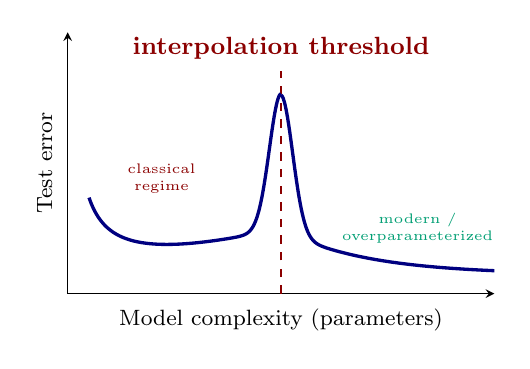
\begin{tikzpicture}
\begin{axis}[
    width=7cm, height=4.9cm,
    xlabel={Model complexity (parameters)},
    ylabel={Test error},
    xlabel style={font=\footnotesize},
    ylabel style={font=\footnotesize},
    tick label style={font=\tiny},
    xmin=0, xmax=10, ymin=0, ymax=6.8,
    grid=major, grid style={gray!15},
    xtick=\empty, ytick=\empty,
    axis lines=left,
    clip=false,
]
    % Interpolation threshold — vertical dashed marker + horizontal label above peak
    \draw[dashed, darkred, thick] (axis cs:5,0) -- (axis cs:5,5.8);
    \node[font=\small\bfseries, darkred, anchor=south]
        at (axis cs:5, 5.85) {interpolation threshold};

    % Single continuous curve: both pieces share the same spike,
    % so the two baselines match at x=5 (peak value ~5.17) and the
    % curve connects without a jump.
    % Classical regime + spike rise
    \addplot[very thick, uzhblue, domain=0.5:5, samples=200]
        {1.5/(x^0.7) + 0.15*(x^1.3) + 3.5*exp(-(x-5)^2/0.15)};
    % Modern regime + spike fall (identical spike term)
    \addplot[very thick, uzhblue, domain=5:10, samples=200]
        {0.5 + 1.17*exp(-0.5*(x-5)) + 3.5*exp(-(x-5)^2/0.15)};

    % Region labels
    \node[font=\tiny, darkred, align=center]
        at (axis cs:2.2, 3.0) {classical\\regime};
    \node[font=\tiny, softgreen, align=center]
        at (axis cs:8.2, 1.7) {modern /\\overparameterized};
\end{axis}
\end{tikzpicture}
\end{center}

\column{0.45\textwidth}
{\footnotesize The classical U turns into a \textbf{second descent} once the model is \emphc{overparameterized}. Three regimes along the curve:

\vspace{0.08cm}
\textcolor{darkred}{\textbf{1. Classical}} ($n_\text{par}\!<\!n_\text{data}$): the familiar bias--variance U --- small models underfit, larger ones chase noise.

\vspace{0.06cm}
\textcolor{darkred}{\textbf{2. Interpolation peak}} ($n_\text{par}\!\approx\!n_\text{data}$): model \emph{just} fits the training set; among all zero-error solutions the optimizer's pick is unstable $\Rightarrow$ variance explodes.

\vspace{0.06cm}
\textcolor{softgreen}{\textbf{3. Modern}} ($n_\text{par}\!\gg\!n_\text{data}$): gradient descent implicitly picks the \emphc{minimum-norm / smoothest} interpolator $\Rightarrow$ it generalizes \emph{better}. More parameters help.

\vspace{0.08cm}
{\scriptsize Belkin et al.\ (2019); Nakkiran et al.\ (2019).}}
\end{columns}

\vspace{0.05cm}
{\footnotesize\emphc{Hands-on:} \texttt{lecture\_04\_B03\_03\_Double\_Descent.ipynb} --- reproduce the curve with random Fourier features.}
\end{frame}
\begin{frame}{}
\begin{center}
{\Huge \textcolor{uzhblue}{Part V}}\\[0.8em]
{\LARGE Advanced Architectures \& Frontiers}
\end{center}
\end{frame}

% --- Slide 48a: Reinforcement Learning in Finance ---
\begin{frame}{Reinforcement Learning in Finance}
\begin{columns}[T]
\column{0.55\textwidth}
\textbf{The RL Loop:}
\begin{itemize}
    \item \textbf{Agent:} Portfolio manager / Algo trader
    \item \textbf{Environment:} The market (prices, order book)
    \item \textbf{State $s_t$:} Current prices, portfolio weights
    \item \textbf{Action $a_t$:} Buy/sell, rebalance
    \item \textbf{Reward $r_t$:} P\&L, Sharpe ratio, utility
\end{itemize}

\vspace{0.2cm}
\textbf{Why not in this course?}
\begin{itemize}
    \item RL finds \emph{strategies} in a \emph{fixed} environment.
    \item We focus on \emph{finding the equilibrium} (the environment itself).
    \item BUT: Critical for hedging \& execution.
\end{itemize}

\column{0.42\textwidth}
\begin{center}
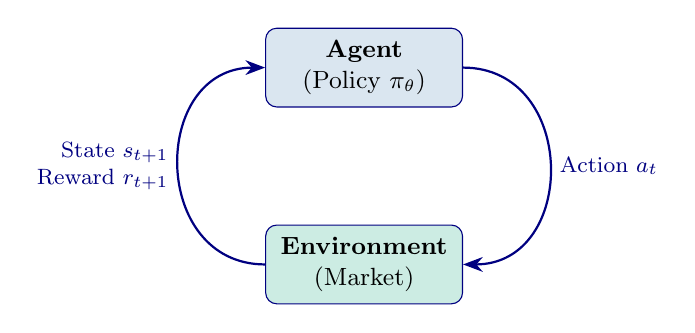
\begin{tikzpicture}[
    box/.style={rectangle, draw=uzhblue, fill=uzhgreylight, rounded corners=4pt,
                minimum width=2.5cm, minimum height=1cm, align=center, font=\small},
    arr/.style={-{Stealth[length=2.5mm]}, thick, uzhblue}
]
    \node[box, fill=softblue!20] (agent) at (0,2.5) {\textbf{Agent}\\(Policy $\pi_\theta$)};
    \node[box, fill=softgreen!20] (env) at (0,0) {\textbf{Environment}\\(Market)};

    \draw[arr] (agent.east) to[out=0,in=0,looseness=1.5] node[midway,right,font=\footnotesize] {Action $a_t$} (env.east);
    \draw[arr] (env.west) to[out=180,in=180,looseness=1.5] node[midway,left,font=\footnotesize,align=right] {State $s_{t+1}$\\Reward $r_{t+1}$} (agent.west);
\end{tikzpicture}
\end{center}
\end{columns}
\end{frame}

% ============================================================================
% Sequence Models mini-section: 9 slides building RNN → LSTM → Transformer
% ============================================================================

% --- Slide S1: Why sequences? ---
\begin{frame}{Why Sequences? Memory Matters}
\footnotesize
\textbf{Many real problems are intrinsically sequential:}
\begin{columns}[T]
\column{0.52\textwidth}
\begin{itemize}\itemsep1pt
    \item \emphc{Next-word prediction:} ``Today we are having a class on deep \rule{0.9cm}{0.4pt}''
    \item \emphc{Time-series forecasting:} inflation, volatility, returns conditional on history
    \item \emphc{Audio / music:} each sample predicted from thousands before (MuseNet, Wav2Vec)
    \item \emphc{Econ application:} Edgeworth cycles in gasoline prices (asymmetric sawtooth)
\end{itemize}

\column{0.46\textwidth}
\textbf{Why an MLP is not enough.}
\begin{itemize}\itemsep1pt
    \item MLP output is \emph{memoryless}: $\hat{y}_t = f(\x_t)$.
    \item Same input $\Rightarrow$ same output, regardless of history.
    \item Sequences have \emph{variable length}; MLPs have a fixed input size.
    \item We need a network that \emphc{carries state across time}.
\end{itemize}
\end{columns}

\vspace{5pt}
\begin{center}
\small
\emphc{Design goals} (Rumelhart et al.\ 1986): \textbf{variable length} $\cdot$ \textbf{order} $\cdot$ \textbf{long-range dependence} $\cdot$ \textbf{parameter sharing across time}.
\end{center}
\end{frame}

% --- Slide S2: From MLP to Recurrence ---
\begin{frame}{From MLP to Recurrence}
\footnotesize
\textbf{Idea.} Give the cell a persistent \emphc{hidden state} $\bm{h}_t \in \R^d$, fed back at every step.

\vspace{2pt}
\begin{columns}[T]
\column{0.55\textwidth}
\begin{itemize}\itemsep1pt
    \item At step $t$, the cell sees \emph{both} the new input $\x_t$ and yesterday's state $\bm{h}_{t-1}$.
    \item Same parameters $\{\W_{hh},\W_{xh},\bb\}$ at every step: \emphc{parameter sharing across time}.
    \item The hidden state $\bm{h}_t$ is a learned summary of the past, the network's ``memory''.
    \item \emph{One} cell processes \emph{any} sequence length.
\end{itemize}

\vspace{3pt}
\begin{center}
{\scriptsize \emphc{RNN is a dynamical system.}  Not a static function.}
\end{center}

\column{0.44\textwidth}
\centering
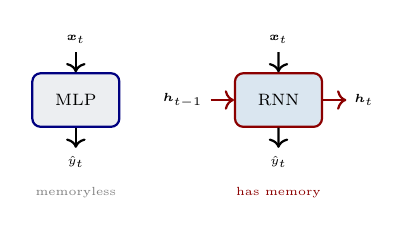
\begin{tikzpicture}[scale=0.85, transform shape, font=\scriptsize,
    m/.style={rectangle, draw=uzhblue, thick, rounded corners=3pt, fill=uzhgreylight,
              minimum width=1.3cm, minimum height=0.8cm, align=center},
    r/.style={rectangle, draw=darkred, thick, rounded corners=3pt, fill=softblue!20,
              minimum width=1.3cm, minimum height=0.8cm, align=center}]
% MLP
\node[m] (mlp) at (0,0) {MLP};
\node[above=0.3cm of mlp, font=\tiny] (xm) {$\x_t$};
\node[below=0.3cm of mlp, font=\tiny] (ym) {$\hat{y}_t$};
\draw[->,thick] (xm) -- (mlp);
\draw[->,thick] (mlp) -- (ym);
\node[below=0.05cm of ym, font=\tiny, gray] {memoryless};

% RNN
\node[r, right=1.7cm of mlp] (rnn) {RNN};
\node[above=0.3cm of rnn, font=\tiny] (xr) {$\x_t$};
\node[below=0.3cm of rnn, font=\tiny] (yr) {$\hat{y}_t$};
\draw[->,thick] (xr) -- (rnn);
\draw[->,thick] (rnn) -- (yr);
\node[font=\tiny, left=0.35cm of rnn] (hin) {$\bm{h}_{t-1}$};
\draw[->,thick,darkred] (hin) -- (rnn);
\node[font=\tiny, right=0.35cm of rnn] (hout) {$\bm{h}_t$};
\draw[->,thick,darkred] (rnn) -- (hout);
\node[below=0.05cm of yr, font=\tiny, darkred] {has memory};
\end{tikzpicture}
\end{columns}
\end{frame}

% --- Slide S3: The RNN cell, unrolled ---
\begin{frame}{The RNN Cell, Unrolled Across Time}
\footnotesize
\begin{columns}[T]
\column{0.44\textwidth}
\textbf{Two equations} define the cell:
\[
\boxed{\;\bm{h}_t = \tanh\!\big(\W_{hh}\,\bm{h}_{t-1} + \W_{xh}\,\x_t + \bb_h\big)\;}
\]
\[
\hat{y}_t = \W_{hy}\,\bm{h}_t + \bb_y
\]

\vspace{4pt}
\begin{itemize}\itemsep1pt
    \item $\bm{h}_0$ initialized to $\bm{0}$ (or learned).
    \item \emphc{Weight sharing:} $\W_{hh},\W_{xh},\W_{hy}$ do not depend on $t$.
    \item A \emph{folded} loop with $T$ steps $\equiv$ an \emph{unfolded} feedforward graph of depth $T$ with \emph{shared} parameters.
\end{itemize}

\column{0.55\textwidth}
\centering
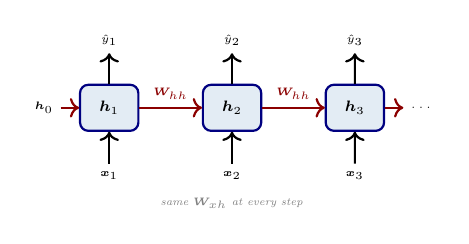
\begin{tikzpicture}[scale=0.78, transform shape, font=\scriptsize,
    c/.style={rectangle, draw=uzhblue, thick, rounded corners=3pt, fill=softblue!15,
              minimum width=0.95cm, minimum height=0.75cm, align=center}]
\foreach \t/\xpos in {1/0, 2/2, 3/4} {
    \node[c] (h\t) at (\xpos,0) {$\bm{h}_\t$};
    \node[font=\tiny] (x\t) at (\xpos,-1.1) {$\x_\t$};
    \node[font=\tiny] (y\t) at (\xpos, 1.1) {$\hat{y}_\t$};
    \draw[->,thick] (x\t) -- (h\t);
    \draw[->,thick] (h\t) -- (y\t);
}
\node[font=\tiny, left=0.3cm of h1] (h0) {$\bm{h}_0$};
\draw[->,thick,darkred] (h0) -- (h1);
\draw[->,thick,darkred] (h1) -- node[above,font=\tiny]{$\W_{hh}$} (h2);
\draw[->,thick,darkred] (h2) -- node[above,font=\tiny]{$\W_{hh}$} (h3);
\node[font=\tiny, right=0.3cm of h3] (hN) {$\cdots$};
\draw[->,thick,darkred] (h3) -- (hN);
\node[font=\tiny, below=0.05cm of x2, gray] {\emph{same $\W_{xh}$ at every step}};
\end{tikzpicture}
\vspace{3pt}
\\
{\scriptsize\emphc{``Same function, many steps.''} Elman (1990); Rumelhart, Hinton \& Williams (1986).}
\end{columns}
\end{frame}

% --- Slide S4: BPTT + vanishing/exploding ---
\begin{frame}{Training: Backpropagation Through Time (BPTT)}
\footnotesize
\textbf{Idea.}  The unrolled RNN is a feedforward net of depth $T$ with \emph{shared} weights.  Run backprop, \emph{sum} weight-gradients across time.

\vspace{3pt}
\begin{columns}[T]
\column{0.56\textwidth}
\textbf{Gradient through time.} For the gradient of $\mathcal{L}_T$ w.r.t.\ an early state $\bm{h}_k$,
\[
\frac{\partial \mathcal{L}_T}{\partial \bm{h}_k} \;=\; \frac{\partial \mathcal{L}_T}{\partial \bm{h}_T} \;\cdot\; \prod_{t=k+1}^{T} \underbrace{\frac{\partial \bm{h}_t}{\partial \bm{h}_{t-1}}}_{=\,\W_{hh}^{\top}\mathrm{diag}(\tanh')}.
\]
A \emphc{long product of the same Jacobian}:
\begin{itemize}\itemsep1pt
    \item If $\|\W_{hh}\|\!>\!1$: gradient \emphc{explodes} $\to$ NaN.
    \item If $\|\W_{hh}\|\!<\!1$: gradient \emphc{vanishes} $\to$ no learning of long-range structure.
\end{itemize}

\vspace{1pt}
{\scriptsize\emphc{Remedies:} gradient clipping, orthogonal init, truncated BPTT, and, most importantly, \emphc{gated cells} (LSTM, GRU).}

\column{0.42\textwidth}
\centering
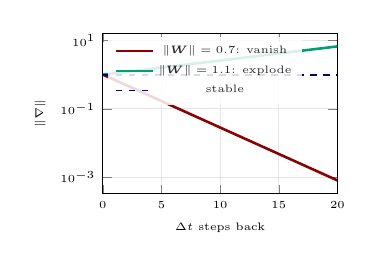
\begin{tikzpicture}[scale=0.78, transform shape, font=\scriptsize]
\begin{axis}[
    width=5.4cm, height=4.2cm,
    xlabel={$\Delta t$ steps back}, ylabel={$\|\nabla\|$},
    xlabel style={font=\tiny}, ylabel style={font=\tiny},
    tick label style={font=\tiny}, ymode=log,
    domain=0:20, samples=40, xmin=0, xmax=20,
    legend style={font=\tiny, at={(0.02,0.98)}, anchor=north west,
                  draw=none, fill=white, fill opacity=0.85},
    grid=both, grid style={gray!20}]
\addplot[darkred, very thick] {0.7^x};
\addlegendentry{$\|\W\|=0.7$: vanish}
\addplot[softgreen, very thick] {1.1^x};
\addlegendentry{$\|\W\|=1.1$: explode}
\addplot[uzhblue, thick, dashed] {1};
\addlegendentry{stable}
\end{axis}
\end{tikzpicture}
\end{columns}
\end{frame}

% --- Slide S5: LSTM ---
\begin{frame}{LSTM: A Memory Conveyor Belt}
\footnotesize
\textbf{Plain-language picture.} A vanilla RNN rewrites its memory at every step.  An LSTM keeps a dedicated \emphc{cell state} $\bm{C}_t$ that mostly flows forward unchanged.

\vspace{2pt}
\begin{columns}[T]
\column{0.54\textwidth}
\textbf{At each date, the cell makes three soft decisions:}
\begin{itemize}\itemsep1pt
    \item \emphc{Forget gate} $f_t$: how much of the old memory survives?
    \item \emphc{Input gate} $i_t$: how much new information should be written?
    \item \emphc{Output gate} $o_t$: how much of memory should be exposed as $\bm{h}_t$?
\end{itemize}

\vspace{2pt}
\[
\bm{C}_t = \bm{f}_t \odot \bm{C}_{t-1} + \bm{i}_t \odot \tilde{\bm{C}}_t,
\qquad
\bm{h}_t = \bm{o}_t \odot \tanh(\bm{C}_t)
\]

\vspace{1pt}
\begin{itemize}\itemsep1pt
    \item \emphc{Key win:} memory changes \emph{additively}, so useful information can survive many steps.
    \item Useful for persistent asymmetric patterns, e.g.\ Edgeworth cycles.
\end{itemize}

\column{0.45\textwidth}
\centering
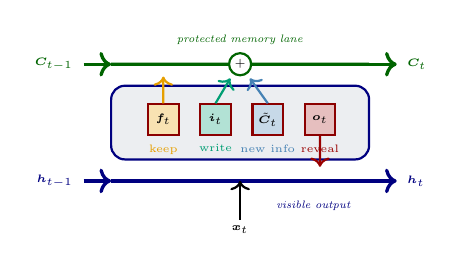
\begin{tikzpicture}[scale=0.78, transform shape, font=\scriptsize,
    cell/.style={rectangle, draw=uzhblue, thick, rounded corners=5pt, fill=uzhgreylight,
                 minimum width=4.2cm, minimum height=1.2cm},
    g/.style={rectangle, draw=darkred, thick, fill=red!10,
              minimum size=0.5cm, font=\tiny, inner sep=1pt},
    plus/.style={circle, draw=darkgreen, thick, fill=white,
                 minimum size=0.36cm, inner sep=0pt, font=\tiny}]
% top lane label — well above the C labels
\node[font=\tiny,darkgreen] at (0,1.35) {\emph{protected memory lane}};
% cell box
\node[cell] (c) at (0,0) {};
% gates centered inside the cell
\node[g, fill=softorange!30] (f) at (-1.25,0.05) {$\bm{f}_t$};
\node[g, fill=softgreen!30]  (i) at (-0.40,0.05) {$\bm{i}_t$};
\node[g, fill=softblue!30]   (u) at ( 0.45,0.05) {$\tilde{\bm{C}}_t$};
\node[g, fill=harvardcrimson!25] (o) at ( 1.30,0.05) {$\bm{o}_t$};
\node[plus] (add) at (0.0,0.95) {$+$};
% Cell-state top lane; C labels inline at the ends
\draw[->, very thick, darkgreen] (-2.55, 0.95) -- (-2.1, 0.95);
\draw[very thick, darkgreen] (-2.1, 0.95) -- (add.west);
\draw[very thick, darkgreen] (add.east) -- (2.1, 0.95);
\draw[->, very thick, darkgreen] (2.1, 0.95) -- (2.55, 0.95);
\node[darkgreen, font=\tiny, anchor=east] at (-2.60, 0.95) {$\bm{C}_{t-1}$};
\node[darkgreen, font=\tiny, anchor=west] at ( 2.60, 0.95) {$\bm{C}_t$};
% Hidden lane; h labels inline at the ends
\draw[->, very thick, uzhblue] (-2.55, -0.95) -- (-2.1, -0.95);
\draw[very thick, uzhblue] (-2.1, -0.95) -- (2.1, -0.95);
\draw[->, very thick, uzhblue] (2.1, -0.95) -- (2.55, -0.95);
\node[uzhblue, font=\tiny, anchor=east] at (-2.60, -0.95) {$\bm{h}_{t-1}$};
\node[uzhblue, font=\tiny, anchor=west] at ( 2.60, -0.95) {$\bm{h}_t$};
% bottom lane label — offset right so it does not clash with the x_t arrow at x=0
\node[font=\tiny,uzhblue] at (1.2,-1.35) {\emph{visible output}};
% gate internal arrows
\draw[->, thick, softorange] (f.north) -- (-1.25,0.75);
\draw[->, thick, softgreen] (i.north) -- (-0.16,0.72);
\draw[->, thick, softblue] (u.north) -- (0.16,0.72);
\draw[->, thick, harvardcrimson] (o.south) -- (1.30,-0.72);
\node[below=0.02cm of f, font=\tiny, softorange] {keep};
\node[below=0.02cm of i, font=\tiny, softgreen] {write};
\node[below=0.02cm of u, font=\tiny, softblue] {new info};
\node[below=0.02cm of o, font=\tiny, harvardcrimson] {reveal};
% x input — enters vertically from below the cell
\node[font=\tiny] at (0,-1.75) {$\x_t$};
\draw[->, thick] (0,-1.58) -- (0,-0.95);
\end{tikzpicture}
\end{columns}

\end{frame}

% --- Slide S6: Limits of recurrence → attention ---
\begin{frame}{Limits of Recurrence $\Rightarrow$ Attention}
\footnotesize
\textbf{Even with LSTMs, two hard limits remain.}

\vspace{3pt}
\begin{columns}[T]
\column{0.5\textwidth}
\textcolor{darkred}{\textbf{1. Sequential $\Rightarrow$ no parallelism.}}
\begin{itemize}\itemsep0pt
    \item Step $t$ must wait for step $t{-}1$.
    \item GPUs love parallelism $\Rightarrow$ RNN training is memory-bound and slow.
    \item Training modern LLMs on $\sim$\,1T tokens with RNNs would take \emph{years}.
\end{itemize}

\column{0.5\textwidth}
\textcolor{darkred}{\textbf{2. Path length blurs long-range signals.}}
\begin{itemize}\itemsep0pt
    \item Information from position 1 reaches position $T$ through $T{-}1$ hops.
    \item Each hop applies a matrix + nonlinearity $\Rightarrow$ fading memory.
    \item Gating helps but does not eliminate path-length decay.
\end{itemize}
\end{columns}

\vspace{6pt}
\begin{center}
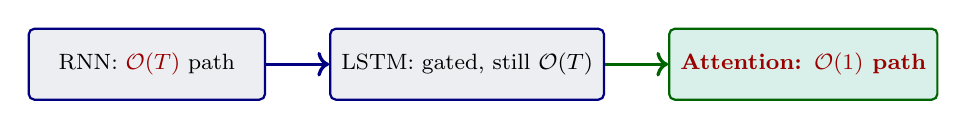
\begin{tikzpicture}[font=\footnotesize,
    b/.style={draw=uzhblue,thick,rounded corners=2pt,fill=uzhgreylight,
              inner sep=4pt,minimum height=9mm,minimum width=30mm,align=center}]
\node[b] (rnn) {RNN: \emphc{$\mathcal{O}(T)$} path};
\node[b,right=8mm of rnn] (lstm) {LSTM: gated, still $\mathcal{O}(T)$};
\node[b,right=8mm of lstm, fill=softgreen!15, draw=darkgreen] (att) {\emphc{\textbf{Attention: $\mathcal{O}(1)$ path}}};
\draw[->,very thick,uzhblue] (rnn) -- (lstm);
\draw[->,very thick,darkgreen] (lstm) -- (att);
\end{tikzpicture}
\end{center}

\vspace{2pt}
{\scriptsize\emphc{Key move.}  Drop recurrence entirely: let every position read every other \emph{directly}, in \emph{parallel}.  This is the \emphc{Transformer} (Vaswani et al.\ 2017).}
\end{frame}

% --- Slide S7: Self-attention intuition ---
\begin{frame}{Self-Attention: Search Inside the Sequence}
\begin{columns}[T]
\column{0.46\textwidth}
{\footnotesize\textbf{Mental model.} Updating token $i$ is like running a search over the whole sequence.}

\vspace{0.08cm}
{\small\textbf{Each token creates three vectors:}}
\begin{itemize}\itemsep0pt
    \item[\textcolor{softblue}{$\blacktriangleright$}] {\footnotesize \textcolor{softblue}{\textbf{Query $q_i$}}: what am I looking for?}
    \item[\textcolor{harvardcrimson}{$\blacktriangleright$}] {\footnotesize \textcolor{harvardcrimson}{\textbf{Key $k_j$}}: what does token $j$ advertise?}
    \item[\textcolor{softgreen}{$\blacktriangleright$}] {\footnotesize \textcolor{softgreen}{\textbf{Value $v_j$}}: what information can token $j$ contribute?}
\end{itemize}

\vspace{0.08cm}
{\small\textbf{Four-step recipe:}}
\begin{enumerate}\itemsep0pt
    \item Add position information.
    \item Compare query $q_i$ with every key $k_j$.
    \item Softmax the scores to get weights $\alpha_{ij}$.
    \item Return a weighted average of the values.
\end{enumerate}

\column{0.52\textwidth}
\centering
{\small\textbf{Worked attention pattern}}

\vspace{0.05cm}
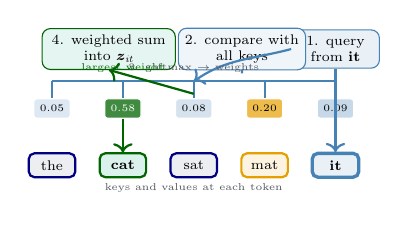
\begin{tikzpicture}[scale=0.72, transform shape, font=\scriptsize,
    tok/.style={rectangle, draw=uzhblue, thick, rounded corners=2pt, fill=uzhgreylight,
                minimum width=0.82cm, minimum height=0.42cm, inner sep=1pt},
    wt/.style={rectangle, draw=white, rounded corners=1pt, minimum width=0.64cm,
               minimum height=0.34cm, inner sep=1pt, font=\tiny},
    box/.style={rounded corners=3pt, align=center},
    lab/.style={font=\tiny, text=uzhgreydark}]
\node[tok] (t1) at (0.0,0.0) {the};
\node[tok, fill=softgreen!14, draw=darkgreen] (t2) at (1.25,0.0) {\textbf{cat}};
\node[tok] (t3) at (2.50,0.0) {sat};
\node[tok, fill=softorange!12, draw=softorange] (t4) at (3.75,0.0) {mat};
\node[tok, fill=softblue!12, draw=softblue, very thick] (t5) at (5.00,0.0) {\textbf{it}};
\node[wt, fill=softblue!18] (w1) at (0.0,1.0) {0.05};
\node[wt, fill=darkgreen!75, text=white] (w2) at (1.25,1.0) {0.58};
\node[wt, fill=softblue!22] (w3) at (2.50,1.0) {0.08};
\node[wt, fill=softorange!70] (w4) at (3.75,1.0) {0.20};
\node[wt, fill=softblue!30] (w5) at (5.00,1.0) {0.09};
\node[draw=softblue, fill=softblue!12, box,
      minimum width=1.55cm, minimum height=0.56cm] (q) at (5.00,2.05) {1. query\\from \textbf{it}};
\node[draw=softblue, fill=softblue!8, box,
      minimum width=1.9cm, minimum height=0.52cm] (cmp) at (3.35,2.05) {2. compare with\\all keys};
\node[draw=darkgreen, fill=softgreen!10, box,
      minimum width=2.35cm, minimum height=0.60cm] (z) at (1.00,2.05)
      {4. weighted sum\\into $\bm{z}_{\textit{it}}$};
\draw[->, thick, softblue] (q.south) -- (t5.north);
\draw[softblue, thick] (0.0,1.48) -- (5.00,1.48);
\foreach \x in {0.0,1.25,2.50,3.75,5.00} {
    \draw[softblue, thick] (\x,1.48) -- (\x,1.18);
}
\draw[->, thick, softblue] (q.west) to[out=195,in=35] (2.50,1.48);
\draw[softblue, thick] (cmp.south) -- (3.35,1.62);
\draw[->, thick, darkgreen] (2.50,1.26) -- (z.south);
\draw[->, thick, darkgreen] (w2.south) -- (t2.north);
\node[lab] at (2.50,1.72) {3. softmax $\rightarrow$ weights};
\node[lab] at (2.50,-0.40) {keys and values at each token};
\node[font=\tiny, darkgreen] at (1.25,1.72) {largest weight};
\end{tikzpicture}

\vspace{0.04cm}
{\scriptsize Blue arrows: build the query and compare it to all keys.  Green arrows: use the weights to pull information, mainly from ``cat'', into $\bm{z}_{\textit{it}}$.}
\\[-1pt]
{\scriptsize Displayed weights: $0.05 + 0.58 + 0.08 + 0.20 + 0.09 = 1.00$.}
\end{columns}
\end{frame}

% --- Slide S8: Transformer block ---
\begin{frame}{From Self-Attention to a Transformer Block}
\footnotesize
\begin{columns}[T]
\column{0.48\textwidth}
\textbf{Matrix form:}
\[
\mathrm{Attn}(Q,K,V) =
\mathrm{softmax}\!\left(\frac{QK^\top}{\sqrt{d_k}}\right)V
\]

\vspace{2pt}
\textbf{Why the extra ingredients?}
\begin{itemize}\itemsep1pt
    \item \textbf{Multi-head attention:} different heads can focus on different relations in parallel.
    \item \textbf{Positional encoding:} attention alone cannot see order, so we add a ruler.
    \item \textbf{Residuals + LayerNorm + MLP:} make deep stacks trainable and expressive.
\end{itemize}
\vspace{2pt}
{\scriptsize\emphc{Econ gloss:} learnable kernel smoothing with learned features and learned similarity.}

\column{0.50\textwidth}
\centering
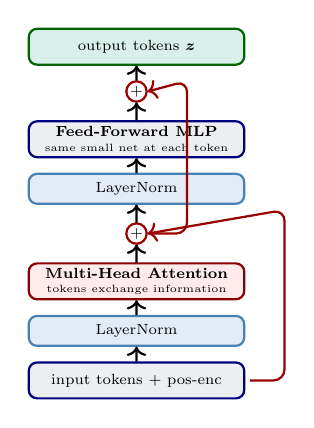
\begin{tikzpicture}[scale=0.76, transform shape, font=\scriptsize,
    b/.style={draw=uzhblue, thick, rounded corners=3pt, fill=uzhgreylight,
              minimum width=3.6cm, minimum height=0.6cm, inner sep=2pt, align=center},
    attn/.style={draw=darkred, thick, rounded corners=3pt, fill=red!8,
              minimum width=3.6cm, minimum height=0.6cm, inner sep=2pt, align=center},
    ln/.style={draw=softblue, thick, rounded corners=3pt, fill=softblue!15,
              minimum width=3.6cm, minimum height=0.5cm, inner sep=2pt, align=center},
    plus/.style={circle, draw=harvardcrimson, thick, fill=white,
                 minimum size=0.34cm, inner sep=0pt, font=\scriptsize}]
\node[b] (in) at (0,0) {input tokens $+$ pos-enc};
\node[ln, above=0.25cm of in] (ln1) {LayerNorm};
\node[attn, above=0.25cm of ln1] (mha) {\textbf{Multi-Head Attention}\\[-1pt]{\tiny tokens exchange information}};
\node[plus, above=0.30cm of mha] (add1) {$+$};
\node[ln, above=0.30cm of add1] (ln2) {LayerNorm};
\node[b, above=0.25cm of ln2] (ff) {\textbf{Feed-Forward MLP}\\[-1pt]{\tiny same small net at each token}};
\node[plus, above=0.30cm of ff] (add2) {$+$};
\node[b, above=0.25cm of add2, fill=softgreen!15, draw=darkgreen] (out) {output tokens $\bm{z}$};
\draw[->,thick] (in) -- (ln1);
\draw[->,thick] (ln1) -- (mha);
\draw[->,thick] (mha) -- (add1);
\draw[->,thick] (add1) -- (ln2);
\draw[->,thick] (ln2) -- (ff);
\draw[->,thick] (ff) -- (add2);
\draw[->,thick] (add2) -- (out);
\draw[->, thick, harvardcrimson, rounded corners=4pt]
    ($(in.east)+(0.08,0)$) -- ++(0.58,0) -- ++(0,2.85) -- (add1.east);
\draw[->, thick, harvardcrimson, rounded corners=4pt]
    ($(add1.east)+(0.08,0)$) -- ++(0.58,0) -- ++(0,2.55) -- (add2.east);
\end{tikzpicture}
\\[1pt]
{\scriptsize\emphc{One block} first mixes information \emph{across tokens}, then transforms each token with an MLP, while skip connections keep deep stacks trainable.}
\end{columns}
\end{frame}

% --- Slide S9: practical takeaway ---
\begin{frame}{RNN, LSTM, Transformer: What to Remember}
\footnotesize
\begin{columns}[T]
\column{0.32\textwidth}
\begin{block}{RNN}
\begin{itemize}\itemsep1pt
    \item Hidden state = running summary of the past
    \item Best first mental model for sequence learning
    \item Hard to train on long histories
\end{itemize}
\end{block}

\column{0.32\textwidth}
\begin{block}{LSTM / GRU}
\begin{itemize}\itemsep1pt
    \item Add gates and a protected memory lane
    \item Strong baseline for specialized time-series tasks
    \item Still sequential, so no large-scale parallelism
\end{itemize}
\end{block}

\column{0.32\textwidth}
\begin{block}{Transformer}
\begin{itemize}\itemsep1pt
    \item Every token can read every other token directly
    \item Full parallelism across positions
    \item Default choice for long-context sequence modeling
\end{itemize}
\end{block}
\end{columns}

\vspace{3pt}
\begin{exampleblock}{Rule of Thumb}
If the pattern is specialized and the history is moderate, an LSTM is still a strong baseline.  If context is long and parallelism matters, start with a Transformer.
\end{exampleblock}

\vspace{1pt}
{\scriptsize Sequence-model notebooks: \texttt{08\_MLP\_LSTM\_Transformer\_Edgeworth\_Cycles} (the three-way comparison on the same task) and \texttt{09\_Transformer\_InContext\_AR1} (advanced / optional).}
\end{frame}

% --- Slide 53: Questions ---
\begin{frame}{}
\begin{columns}[c]
\column{0.45\textwidth}
\begin{center}

\includegraphics[width=0.85\textwidth]{figures/quest.png}
\end{center}

\column{0.50\textwidth}
\begin{center}
{\Huge \textcolor{uzhblue}{\textbf{Questions?}}}

\vspace{0.8cm}
{\large Simon Scheidegger}\\[4pt]
{\small HEC, University of Lausanne}\\[4pt]
\url{https://sischei.github.io}

\vspace{0.6cm}
{\small Materials:~~\url{https://github.com/sischei/Deep_Learning_for_Solving_And_Estimating_Dynamic_Economic_Models}}
\end{center}
\end{columns}
\end{frame}

\end{document}
